\documentclass[11pt]{article}
\usepackage[margin=1in]{geometry}
\usepackage{amsmath,amssymb}
\usepackage{graphicx}
\usepackage{booktabs}
\usepackage[numbers,sort&compress]{natbib}
\usepackage{authblk}
\usepackage[hidelinks]{hyperref}
\hypersetup{pdftitle={From Material Turnover to Causal Memory: A Prospective Falsification Ladder for Organizational Continuity in a Simulated Droplet},pdfauthor={Autonomous research agent (see AI-authorship disclosure)},pdfsubject={Organizational memory, material turnover, causal identity in a simulated reaction-transport droplet},pdfkeywords={organizational memory; material turnover; causal identity; reaction-transport; prospective falsification}}
\usepackage{caption}
\captionsetup{font=small}
\renewcommand{\arraystretch}{1.15}
\title{\textbf{From Material Turnover to Causal Memory: A Prospective Falsification Ladder for Organizational Continuity in a Simulated Droplet}}
\author[1]{[AUTHOR NAME REQUIRED]}
\affil[1]{[AFFILIATION REQUIRED] \quad ORCID: [ORCID IF AVAILABLE]}
\date{July 2026 \quad (V3: statistical re-audit; scope of causal and second-coordinate claims corrected)}
\begin{document}
\maketitle

\begin{abstract}
\noindent Biological individuals persist while their constituent material is continually replaced, which motivates
the idea that \emph{organization}, rather than matter, is a substrate of biological memory and identity. We ask a
deflationary, falsifiable version of this question in a simulated reaction--transport droplet endowed with a designed
two--component intensive memory field $m=(m_1,m_2)$ coupled to nutrient uptake ($m_+=m_1+m_2$) and attractant
production ($m_-=m_1-m_2$). Over a preregistered ladder of interventions evaluated prospectively, (and, we stress at the outset, without any claim of individual identity), with grouped
leave--history--out statistics, sealed hold--out families, kill--switches, and continuity--safe entity tracking, we
establish one positive result and a matched negative boundary. \textbf{Positive:} under a globally imposed nutrient
history, many persistent droplets locally encode a similar engineered cumulative--experience coordinate $h_1$; a
\emph{continuously tracked} droplet retains this internal causal state through substantial constituent turnover
(longitudinal hold--out on untouched seeds: $h_1$ held--out $R^2=0.98$, $95\%$ CI $[0.97,1.00]$ at old--material
fraction $M\approx0.19$, with $36/36$ track survival), $h_1$ is causally expressed in the interventional sense that the memory--inert and erase controls carry no history information (deterministically), with a positive but statistically uncertain sufficiency magnitude (transplant $R^2=0.61$, $95\%$ CI $[-0.69,0.87]$ at $n=12$); its \emph{retention} through deep turnover is the robustly established result ($R^2=0.98$, $95\%$ CI $[0.97,1.00]$).
Crucially $h_1$ is \emph{global} in informational content: it is decodable from essentially any large droplet, and
therefore does \textbf{not} individuate droplets. \textbf{Negative:} a second initially decodable coordinate $h_2$ (temporal order / value dispersion) has an $\approx$one--dimensional causal response, and its deep--turnover retention is \emph{not established}: the held--out estimate ($R^2=0.34$) carries a wide $95\%$ confidence interval ($[-0.89,0.87]$) that spans the $0.50$ certification threshold, so at $n=12$ histories it is neither confirmed nor refuted. Our methodological contribution is a
falsification ladder that separates decodability, storage, causal expression, material--turnover survival,
longitudinal continuity, and individuation, together with a transparent correction chain (grouped--evaluation
leakage; seed--family instability; statistical power; largest--component reselection versus continuity--safe
tracking). We claim no life, agency, identity, individuation, reproduction, or heredity.
\end{abstract}

\section{Introduction}
An organism replaces most of its molecules many times over its life, yet remains, in a functional sense, the same
individual. This everyday fact underlies a family of ideas --- from cybernetics and autopoiesis to contemporary
theories of biological individuality --- in which persistence of \emph{organization} rather than of \emph{matter}
is treated as a candidate substrate for biological memory and identity \citep{ashby1952,maturana1980,godfreysmith2009}.
If an organized, self--maintaining entity could record aspects of its history in a way that outlives its
constituent material, that record would be a natural minimal model of organizational memory. Our goal in this
paper is to render this intuition precise, testable, and --- where the evidence demands --- falsifiable, in a
tractable simulation.

We adopt three deliberately stringent criteria for what should count as a memory of experience, as opposed to a
mere statistical shadow of it. First, a history variable being \emph{decodable} from a system is not sufficient: a
decoder can exploit residual environment, current body size, laboratory--frame position, or simply the fact that a
globally imposed history is written similarly into every entity in the world. Decodability is necessary but weak.
Second, a memory worth the name must be \emph{causal}: it must shape the system's dynamics, in the interventionist
sense that ablating or transplanting it changes downstream physical behaviour \citep{pearl2009,rubin1974,pearl1995}.
Third, if the memory is to be \emph{organizational} rather than merely material, it must survive substantial
replacement of the constituent material of the entity that carries it. To these we add a fourth, sharper property
that is often conflated with the third: \emph{individuation}, i.e.\ whether the memory makes one entity
distinguishable from another by its particular history. Individuation requires strictly more than persistence, and
we do not claim it here.

These criteria motivate an experimental programme rather than a single measurement. Decodability, causal
expression, and turnover survival can each hold or fail independently, and an honest evaluation must test them
separately and prospectively. We therefore construct a ``falsification ladder'': a sequence of preregistered
experiments, each with a sealed prospective family and an explicit pass/fail gate, that climbs from the weakest
property (decodability at rest) toward the strongest (a causal, transplantable, turnover--surviving,
history--individuating coordinate). At each rung we attempt to break the positive reading with the strongest
available trivial explanation before accepting it, and we retain and report negative results as first--class
outcomes.

The system we study is a simulated ``scaffold'' droplet: a periodic two--dimensional reaction--transport medium in
which a localized, viable, self--maintaining density field advects toward a self--produced attractant, grows on a
nutrient, and dies. On top of a frozen version of this substrate we engineer a bounded, distributed memory field
that is written by a local experience signal, maintained on two timescales, inherited by newly grown material, and
read back through two pre--existing physical channels (uptake and attractant production). We stress from the outset
that this memory is \emph{engineered}, not emergent: our contribution is not a new memory mechanism but a
disciplined test of the \emph{causal and material status} of a history coordinate carried by such a mechanism under
turnover, and a demonstration of how several plausible positive readings fail.

Two results anchor the paper. The first is positive but carefully scoped: a one--dimensional cumulative--experience
coordinate, which we call $h_1$, is prospectively decodable, causally expressed through uptake, transplantable into
a fresh standardized body, and --- when a single droplet is followed with a continuity--safe tracker --- retained
through the replacement of roughly four--fifths of its material. However, because the driving history is imposed
globally, $h_1$ is decodable from essentially any large droplet in the world; it is a memory of the world's history
carried locally, not a marker of individual identity. The second result is a matched negative boundary: a second
coordinate $h_2$, encoding temporal order, is decodable at rest but fails to qualify as an independent, causal,
turnover--surviving dimension. The interplay of these two results, and the corrections required to reach them,
constitute the paper's contribution.

A methodological theme runs throughout. Reaching the scoped positive and the clean negative required correcting
several seductive errors: a replicate--leaking cross--validation that inflated an apparent high--dimensional
result \citep{kaufman2012}; a single seed family whose behaviour did not generalize; an underpowered deep--turnover
estimate; and --- exposed by a collaborator's visual inspection of an animation --- a largest--component
\emph{reselection} tracker that manufactured spurious entity continuity. We treat these corrections not as
embarrassments but as the empirical substance of a falsification ladder, and we devote explicit methods and results
subsections to the tracking correction because it changed the scientific record.

To make the programme concrete, we frame six competing readings that any candidate coordinate must survive, and we
attach an experiment to each. A coordinate could be (i) a genuine causal, transplantable, turnover--surviving,
individuating memory; or it could be a mere (ii) material residue carried by the original constituents, (iii)
environmental residue read from persistent nutrient or attractant fields, (iv) laboratory--frame artefact exploiting
absolute position or orientation, (v) measurement artefact visible only through an inadequate readout, or (vi) a
stored but causally silent pattern. These readings are not rhetorical: each makes a distinct, falsifiable prediction
under a specific control (turnover, environmental reset, translation/rotation, alternative readout, targeted
ablation), and much of the paper consists of executing those controls. The discipline of naming the trivial
explanations \emph{before} testing, and of trying hardest to confirm them, is what separates a falsification ladder
from a search for a positive result.

Throughout, we distinguish sharply between what is \emph{observed} (a decode value, a confidence interval, an
ablation contrast), what is \emph{inferred} (a mechanistic reading consistent with the observations), and what
remains \emph{speculative} (an interpretation not yet tested). We also distinguish the \emph{writing--map} capacity
(the rank of the map from history to stored memory), the \emph{memory--state} dimensionality (the rank of the
stored field), the \emph{observability} of a coordinate (whether a decoder can read it at a chosen window), and the
\emph{causal--response} dimensionality (how many independent axes the memory drives in the physics). Conflating
these four is the single most common way to over--read a positive decode, and keeping them separate is a
precondition for the corrections we report. We work in simulation deliberately. A wet--lab protocell offers physical realism but poor experimental control: one cannot erase a droplet's memory exactly, transplant an internal state into a standardized body, ablate a single readout channel while holding everything else fixed, or replay a trajectory deterministically. These operations --- which distinguish a causal memory from a correlate --- are trivial in a frozen simulator and are why a simulation can answer the causal and material questions more sharply than a physical system can, at the cost of realism. The trade is explicit: we buy interventional and statistical rigor and pay with simulator specificity, and we return to the substrate--versus--architecture question in the discussion.

\section{Related work}
Our substrate belongs to the long tradition of reaction--diffusion and dissipative pattern formation initiated by
\citet{turing1952} and developed through activator--inhibitor theory \citep{gierer1972}, positional information
\citep{wolpert1969}, and the modern synthesis of nonequilibrium pattern formation \citep{cross1993,kondo2010,nicolis1977}.
The local excitable chemistry we use is of FitzHugh--Nagumo type \citep{fitzhugh1961,nagumo1962}. Unlike this
literature, our interest is not the patterns themselves but a superimposed, bounded memory field and its causal and
material status.

The memory we engineer is an attractor--like internal state. Distributed attractor memories are classical in
theoretical neuroscience \citep{hopfield1982}, and the dynamical--systems notions of attractors and observability
frame what it means for a hidden state to be recoverable and consequential \citep{strogatz1994,hermann1977}. We
borrow the vocabulary of observability but reach a deflationary conclusion: recoverability of a hidden coordinate
is not, by itself, evidence of individual memory.

At the biological end, our droplet is a caricature of an active droplet or protocell --- an idealized model \emph{inspired by}, not quantitatively corresponding to, such systems. Chemically active droplets can
grow and divide in ways reminiscent of cell proliferation \citep{zwicker2017}, liquid--liquid phase separation
organizes intracellular biochemistry into condensates \citep{brangwynne2009,hyman2014,banani2017}, and minimal
protocells can encapsulate, grow, and divide \citep{szostak2001,hanczyc2003}. Recent experimental systems sharpen this contrast: active coacervate droplets are chemically driven condensates whose components \emph{turn over} out of equilibrium \citep{nakashima2021}; peptide coacervates can \emph{proliferate} by recursive growth and division \citep{matsuo2021}; and synthetic protocells can undergo history--dependent \emph{differentiation} into distinct internal states \citep{higashi2025}. These works establish, in real chemistry, turnover, proliferation, and state change, but they characterize physical or compositional dynamics rather than asking whether an internal coordinate is a \emph{decodable, causally--tested, turnover--surviving} record of experience evaluated prospectively with intervention and continuity--safe tracking. That measurement question, at frozen physics, is our contribution; the comparison also bounds our result --- unlike \citet{higashi2025} we neither implement nor demonstrate differentiation into distinct per--droplet states. Molecular biology
does provide concrete memory mechanisms --- bistable genetic and chemical switches with hysteresis
\citep{gardner2000,elowitz2000,ferrell2002,ptashne2004} --- and we use these as a conceptual benchmark for what a
qualified second, independent memory dimension would look like, and as motivation for why our (failed) $h_2$ would
have needed bistable, protected maintenance rather than passive linear averaging to persist.

Conceptually, the paper engages theories of biological individuality and organizational identity
\citep{godfreysmith2009,varela1974,maturana1980,ashby1947,ashby1952} and the artificial--life programme's open
problems around the emergence and persistence of individuals \citep{bedau2000}. Our stance is empirical and
deflationary: rather than argue for a definition of individuality, we operationalize necessary conditions
(causality, transplantability, turnover survival, individuation) and test them. Methodologically we lean on causal
inference \citep{pearl2009,rubin1974,pearl1995}, the bootstrap for grouped uncertainty \citep{efron1979},
preregistration and falsification \citep{nosek2018,popper1959}, the theory of leakage in predictive evaluation
\citep{kaufman2012}, and classical connected--component and particle--tracking methods \citep{rosenfeld1966,jaqaman2008},
the last of which is central to the tracking correction we report.

Two contrasts with prior modelling deserve emphasis. First, in the active--droplet and protocell literature the
object of interest is typically the \emph{physical} life cycle --- growth, shape instability, division
\citep{zwicker2017,hanczyc2003} --- and memory, when discussed, is chemical composition rather than a decodable,
causally--tested history coordinate. We instead hold the physics frozen and ask a measurement question about an
engineered internal coordinate, which lets us apply the machinery of prospective evaluation and causal intervention.
Second, in synthetic biology, durable memory is achieved by \emph{bistable} circuits whose hysteresis protects a
state across perturbation and division \citep{gardner2000,elowitz2000,ferrell2002}. Our maintenance terms are, by
contrast, linear and averaging; the comparison predicts --- correctly, as it turns out --- that a dispersion--coded
second coordinate should not survive turnover, and it points to bistable maintenance as the missing ingredient. The observability lens clarifies why the two coordinates behave so differently under turnover \citep{hermann1977}. The cumulative coordinate $h_1$ is encoded in the \emph{level} of the memory, a quantity that growth and uniform death preserve and that the smoothing terms do not erase; it is therefore robustly observable through turnover. The order coordinate $h_2$ is encoded in the \emph{dispersion} of the memory, a quantity that linear low--pass maintenance and fresh, history--independent growth actively degrade; it is therefore observable at rest but not through deep turnover. We offer this as a \emph{hypothesis} rather than an established mechanism (the smoothing--ablation and dispersion--growth results above caution against a purely linear--averaging account); whether a bistable, hysteretic maintenance rule would protect such a distinction \citep{gardner2000,ferrell2002,ptashne2004} is a question for future work, not a result of this paper. In
this sense the negative result is not merely a null; it is interpretable against an established mechanistic
benchmark. The conceptual target --- persistence of an individual through material replacement --- is old, from the ship of Theseus to the observation that most somatic constituents turn over on timescales far shorter than an organism's life. Modern philosophy of biology distinguishes physiological individuality (a cohesive self--maintaining metabolic unit) from evolutionary individuality (a unit of selection with reproduction and heredity) \citep{godfreysmith2009}, and organizational accounts locate identity in a self--producing organization rather than its matter \citep{varela1974,maturana1980}. Our droplet speaks only to a minimal physiological notion: whether a self--maintaining unit can carry a causal record of its experience across turnover. It says nothing about evolutionary individuality, which requires reproduction and heredity that we neither implement nor claim; a turnover--surviving causal state is sometimes over--read as evidence of the evolutionary notion, and our results support only the weaker reading, for a globally shared history. We are explicit about novelty. The mechanism ($m_+$/$m_-$ readouts, two--timescale integration) is engineered and modest; we do not present it as a new memory principle. The contribution is the disciplined \emph{evaluation}: a prospective, kill--switched falsification ladder that repeatedly resists the temptation to over--read a positive decode, together with a transparent chain of corrections --- replicate leakage, seed--family instability, statistical power, and largest--component reselection --- each of which is a recurring hazard in computational studies of simulated organisms. A reader who takes nothing else from the paper should take the methodological pattern: intervene, group, seal, power, track, and preregister a stopping rule, so that a marginal signal cannot be inflated into a claim of individual memory or life.

\section{Model}
\label{sec:model}
The substrate is a periodic $64\times64$ lattice evolved with timestep $\mathrm{d}t=0.1$ (Table~\ref{tab:state},
Table~\ref{tab:params}). It carries a coarse density field $\rho(x,t)$, an internal excitable chemistry $(U,V)$, a
diffusing nutrient $N$, and a self--produced attractant $c$. Density is transported advectively up attractant
gradients, grows where nutrient is available and crowding is low, and decays; the internal $(U,V)$ chemistry follows
a FitzHugh--Nagumo--type excitable law \citep{fitzhugh1961,nagumo1962}. This ``scaffold'' is frozen throughout the
paper (its implementation hash is recorded in the reproducibility appendix); all experiments only add or read a
memory field on top of it, or intervene on that memory.

\paragraph{Memory writing.} The engineered memory is a bounded intensive field $m=(m_1,m_2)$, stored extensively as
$M_f=\rho\,m$ so that it is transported with the density exactly as the internal chemistry is. It is written by a
local experience signal
\begin{equation}
\Psi \;=\; \tanh\!\big(k_{\exp}\,(N-c) \;+\; k_{\mathrm{up}}\,(\text{uptake}-\overline{\text{uptake}})\big),
\label{eq:psi}
\end{equation}
which compares local nutrient to attractant and local uptake to its spatial mean, so that $\Psi$ encodes a bounded
``how nutritive and how surprising is it here'' signal. Each memory component is a leaky integrator of $\Psi$ with
its own forgetting timescale, together with local templating toward a neighbourhood consensus and weak diffusion:
\begin{equation}
\dot m_k \;=\; \eta_w\,\Psi \;-\; \eta_{d,k}\,m_k \;+\; \eta_t\big(\langle m_k\rangle_{\mathrm{nbr}}-m_k\big)
\;+\; D_m\,\nabla^2 m_k, \qquad m_k \in [-1,1],\quad k\in\{1,2\}.
\label{eq:write}
\end{equation}
The two components differ only in their forgetting rate ($\eta_{d,1}\gg\eta_{d,2}$; a fast and a slow integrator).
Newly grown material inherits the local intensive memory, $M_f \mathrel{+}= g\,m$ (with $g$ the local growth), and
death scales all fields uniformly; consequently growth and death approximately \emph{preserve} the intensive
memory, a fact that matters for the turnover analysis.

\paragraph{Memory readout.} The memory is read through two pre--existing physical channels via the sum and
difference coordinates $m_+=m_1+m_2$ and $m_-=m_1-m_2$:
\begin{align}
\text{uptake} &\;\to\; \text{uptake}\,\big(1+\lambda_+\tanh m_+\big), \label{eq:readplus}\\
\text{attractant production} &\;\propto\; 1+\lambda_-\tanh m_-. \label{eq:readminus}
\end{align}
With $\lambda_-=0$ the model reduces bit--identically to a single--channel predecessor, and with
$\lambda_+=\lambda_-=0$ it reduces to the frozen scaffold; these exact reductions are used as backward--compatibility
tests. The two readouts are the only causal pathways from memory to physics.

\paragraph{History coordinates.} Experience is imposed as a two--phase \emph{global} nutrient history: during an
early phase the whole field receives $N\mathrel{+}=a_{\mathrm{early}}$ per step for $T$ steps, and during a late
phase $N\mathrel{+}=a_{\mathrm{late}}$ for $T$ steps. From the two phase amplitudes we define two orthogonal history
coordinates,
\begin{equation}
h_1 \;=\; a_{\mathrm{early}}+a_{\mathrm{late}} \quad(\text{cumulative dose}), \qquad
h_2 \;=\; a_{\mathrm{late}}-a_{\mathrm{early}} \quad(\text{temporal order}),
\label{eq:coords}
\end{equation}
sampled independently over a viable amplitude band (Table~\ref{tab:histories}). Because the drive is global, every
droplet in the world experiences the same $(h_1,h_2)$; the decoding task across a family therefore tests whether the
\emph{world's} history is written into local memory, not whether droplets carry \emph{distinct} histories.

\paragraph{Scaffold dynamics and boundary conditions.} The frozen scaffold combines four ingredients. Transport is
advective toward the self--produced attractant, so density accumulates where $c$ is high, producing localized,
motile droplets rather than a spread film. Growth is nutrient--limited and crowding--limited, $g\propto \rho\,N\,
\max(0,1-\rho/\rho_{\max})$, so entities saturate in size; death is a uniform decay. The internal $(U,V)$ chemistry
is excitable \citep{fitzhugh1961,nagumo1962}, giving each droplet a bounded internal state that co--moves with the
density. All fields are periodic in both directions, which is important for the tracking analysis: a droplet may
straddle a boundary and appear at both edges while remaining a single connected component under wrap--aware
labelling \citep{rosenfeld1966}. Because the memory is stored extensively as $M_f=\rho\,m$ and advected, diffused,
and inherited exactly as $U,V$ are, it is a bona fide internal field of the droplet rather than an externally
imposed label; in particular no entity identity, cohort index, seed number, or history label ever enters
Eqs.~\eqref{eq:psi}--\eqref{eq:readminus}. This ``no--leakage'' property is enforced by construction and checked in
every experiment. Two additional integrity tests bracket every result. Backward--compatibility: setting $\lambda_-=0$ reproduces the single--channel predecessor bit--identically, and setting $\lambda_+=\lambda_-=0$ reproduces the frozen scaffold, so any measured effect is attributable to the memory coupling and not to an incidental change in the base dynamics. No--leakage: because history labels, cohort indices, seeds, and entity identities never enter Eqs.~\eqref{eq:psi}--\eqref{eq:readminus}, a positive decode cannot be an artefact of a smuggled identity variable; the pulse--chase tracer that quantifies turnover is likewise inert, re--binning a passive cohort field without touching $\rho,U,V,N,c$.
\begin{table}[t]\centering\small
\caption{State variables of the frozen scaffold and the engineered memory.}
\label{tab:state}
\begin{tabular}{@{}lll@{}}\toprule
symbol & type & interpretation\\\midrule
$\rho$ & field & coarse density of the droplet material\\
$U,V$ & fields & internal excitable chemistry (FitzHugh--Nagumo type)\\
$N$ & field & diffusing nutrient (globally driven by the history)\\
$c$ & field & self--produced diffusing attractant\\
$m=(m_1,m_2)$ & field & engineered intensive memory (fast / slow)\\
$M_f=\rho\,m$ & field & extensive memory, transported with $\rho$\\
cohort $C$ & field & passive pulse--chase tracer (never enters dynamics)\\\bottomrule
\end{tabular}
\end{table}
\begin{table}[t]\centering\small
\caption{Frozen C1c parameters (the selected writing configuration; unchanged in all reported analyses).}
\label{tab:params}
\begin{tabular}{@{}lll@{}}\toprule
symbol & value & meaning\\\midrule
$\eta_w$ & $0.015$ & experience write gain\\
$\eta_{d,1},\ \eta_{d,2}$ & $0.35,\ 0.006$ & fast / slow forgetting rates\\
$\eta_t$ & $0.010$ & local templating (4--neighbour consensus)\\
$D_m$ & $0.010$ & memory diffusion coefficient\\
$k_{\exp},\ k_{\mathrm{up}}$ & $1.0,\ 1.0$ & experience--signal gains in Eq.~\eqref{eq:psi}\\
$\lambda_+,\ \lambda_-$ & $0.25,\ 0.15$ & uptake / attractant coupling in Eqs.~\eqref{eq:readplus}--\eqref{eq:readminus}\\
grid,\ $\mathrm{d}t$ & $64\times64$,\ $0.1$ & lattice, timestep\\\bottomrule
\end{tabular}
\end{table}

\section{Experimental methodology}
\label{sec:methods}
\paragraph{Protocol.} Each trial warms a body from a random seed for $2000$ steps, erases the memory
($M_f=0$), applies a two--phase history (Eq.~\ref{eq:coords}; $T=60$ per phase), settles for $20$ steps, then
relabels all extant material as ``old'' (cohort $0$) and evolves the frozen dynamics forward with no further
drive; material grown thereafter is ``new'' (cohort $1$). The old--material fraction
$M=\text{mass}_{\text{old}}/\text{mass}_{\text{total}}$ of the tracked entity quantifies turnover; the pulse--chase tracer is passive and never enters $\rho,U,V,N,c$ (``turnover'' here is a bookkeeping construct on a passive cohort field, not a chemical exchange process) \citep{jaqaman2008}. Interventions comprise erasure ($M_f=0$),
mean--field and structured transplant into a standardized erased recipient body, channel--specific readout ablation
($\lambda_+\!\to\!0$ or $\lambda_-\!\to\!0$), and an exact--clone / stochastic ceiling (Table~\ref{tab:interventions}).

\paragraph{Entity detection and tracking.} The substrate self--organizes into many small droplets. Connected
components are labelled with a periodic (wrap--aware) algorithm and summarized by circular centroids (a \emph{viable} entity is a single localized connected component above a minimum size threshold)
\citep{rosenfeld1966}; all memory features used for decoding are permutation--invariant statistics of the memory
values over an entity's cells and are therefore translation-- and reflection--invariant by construction, a property
we verify directly (\S\ref{sec:tracker}). The historical analyses selected, at each checkpoint, the \emph{largest}
connected component. As we show in \S\ref{sec:tracker}, this is a per--frame \emph{reselection} rule, not
longitudinal tracking; we therefore additionally define a frozen longitudinal tracker that initializes once and
thereafter follows the entity of maximum periodic mask overlap, censoring the track on loss and never using $h_1$,
$h_2$, $M$, or any history label in its matching. All turnover claims are re--certified with this tracker.

\paragraph{Decoding and statistics.} History coordinates are decoded from internal memory by ridge regression with
grouped \emph{leave--history--out} cross--validation: all replicate rows that share a history (across seeds) are
held out together, so no replicate of a held--out history remains in training. This is essential because row--wise
leave--one--out leaks through shared replicates and inflates apparent performance \citep{kaufman2012}. Development
and prospective families are strictly separated; prospective families are generated and SHA--256--hashed before any
selection and executed exactly once (Table~\ref{tab:families}); uncertainty is quantified by donor--level
bootstrap $95\%$ confidence intervals \citep{efron1979}; and every primary decode is compared against constant,
shuffled--history, and same--law/different--seed nulls. Causal claims use interventions in the potential--outcomes
and graphical sense \citep{rubin1974,pearl1995,pearl2009}: an effect is causal if it changes under erasure,
transplant, or channel ablation and collapses under a memory--inert control. Preregistration and explicit
pass/fail kill--switches \citep{nosek2018,popper1959} bound the programme so that mechanism development cannot
continue indefinitely.

\paragraph{Decoder and score.} For a history family we aggregate replicate rows to the history level and predict a
coordinate $y\in\{h_1,h_2\}$ from a fixed feature vector $\phi$ (permutation--invariant memory statistics) by ridge
regression, reporting the grouped leave--one--history--out coefficient of determination
\begin{equation}
R^2 \;=\; 1 - \frac{\sum_i (y_i-\hat y_{-i})^2}{\sum_i (y_i-\bar y)^2},
\label{eq:r2}
\end{equation}
where $\hat y_{-i}$ is the prediction for history $i$ from a model fit on all other histories. Preprocessing
(centering, scaling, near--constant--column removal) is fit on the training fold only. Confidence intervals are
obtained by resampling histories (donors) with replacement \citep{efron1979}. A coordinate is deemed decodable only
if $R^2$ exceeds the constant, shuffled--history, and same--law/different--seed nulls, and, for certification, only
if the lower confidence bound exceeds the preregistered threshold.

\paragraph{Longitudinal tracker.} From the initial largest entity with cell set $S_0$, the tracked entity at the
next update is
\begin{equation}
S_{t+1} \;=\; \arg\max_{S\in \text{components}} \; \frac{|S \cap S_t|}{|S_t|},
\qquad \text{lost if } \max_S \frac{|S\cap S_t|}{|S_t|} < \theta,
\label{eq:track}
\end{equation}
with overlap threshold $\theta=0.1$; a tie within $10\%$ marks the track \emph{ambiguous} and censors it. The score
in Eq.~\eqref{eq:track} depends only on geometry, never on $h_1$, $h_2$, $M$, or labels. Splits are handled by
following the maximum--overlap fragment; merges keep the maximum--overlap component and are recorded as events.
Longitudinal metrics are reported only for uncensored tracks, so a lost entity is never silently replaced by another. The overlap threshold $\theta=0.1$ was fixed before the hold-out; the certification is insensitive to $\theta\in[0.05,0.2]$ because a surviving entity's frame-to-frame overlap greatly exceeds $\theta$ except at genuine loss.

\paragraph{Kill--switch and power.} Before the deep--turnover certification we performed a development--only power
analysis: from pilot variance components we asked what sample size could place a lower confidence bound above the
threshold under alternatives $R^2\in\{0.50,0.65,0.75\}$. A pilot point estimate at or below the threshold does \emph{not} imply the true value is below threshold, nor that no future sample could exceed it; additional donor histories could move the estimate either way. What the pilot established was only that, at $n=12$, the deep--turnover $h_2$ estimate is too uncertain to certify. Deciding the question would require substantially more donor histories, which we did not run. The frozen
prospective sample was fixed accordingly, and the family was executed once. \paragraph{The experimental sequence.} The results below are the outcome of nine sequential experiments; for each, the protocol and the sealed prospective family were committed to version control before that experiment's prospective family was executed (Table~\ref{tab:provenance}), an autonomous rapid workflow rather than classical multi--week preregistration. (1) A material--continuity experiment established that the droplet persists under turnover but that a snapshot nearly suffices to predict its future, i.e.\ no strong history--specific hidden persistence. (2) A hidden--state experiment showed the internal state is a generic causal attractor, not an individuating fingerprint. (3) An organizational--memory experiment introduced the designed two--component field and showed it causal, erasable, transplantable, with a readout that collapsed onto one cumulative coordinate. (4) A multi--channel experiment added the $m_-\!\to$attractant readout and made temporal order causally readable. (5) A writing--dimensionality audit corrected an apparent high--dimensional storage via grouped evaluation. (6) A writing redesign (C1c) produced two decodable coordinates at rest but a one--dimensional causal response. (7) A spatial--memory experiment characterized $h_2$ as a frame--free dispersion and first reported a turnover collapse. (8) A maintenance experiment corrected that report --- the collapse was family--dependent and underpowered, the loss neither homogenization nor dilution --- but did not certify deep survival. (9) A final kill--switch found that, at $n=12$ histories, $h_2$ deep--turnover retention did not meet the certification criterion and is not established (the held--out CI spans the threshold; §\ref{sec:results}). The tracker--continuity audit then re--certified all turnover claims longitudinally.

\begin{table}[t]\centering\small
\caption{Causal--intervention conditions.}
\label{tab:interventions}
\begin{tabular}{@{}lp{5.6cm}l@{}}\toprule
condition & operation & tests\\\midrule
erase & set $M_f=0$ & memory necessity\\
mean transplant & copy entity--mean $(m_1,m_2)$ into fresh body & transplantability (scalar)\\
structured transplant & copy entity--relative pattern into fresh body & spatial transplantability\\
$\lambda_+\!\to\!0$ & disable the uptake readout & channel specificity (uptake)\\
$\lambda_-\!\to\!0$ & disable the attractant readout & channel specificity (attractant)\\
both $\to 0$ & memory--inert control & causal necessity (all channels)\\
exact clone & re--run under bounded environmental noise & stochastic ceiling\\\bottomrule
\end{tabular}
\end{table}
\begin{table}[t]\centering\small
\caption{History families (each two--phase; amplitudes sampled independently in the stated band).}
\label{tab:histories}
\begin{tabular}{@{}llll@{}}\toprule
family & phase amplitude band & purpose & $h_1,h_2$\\\midrule
$F_{\mathrm{mid}}$ & $[0.003,0.020]$ & viable, mildly saturating & Eq.~\eqref{eq:coords}\\
$F_{\mathrm{low}}$ & $[0.001,0.008]$ & more graded (capacity--viability map) & Eq.~\eqref{eq:coords}\\
matched--dose (order) & phase--swapped $N{\to}c$ vs $c{\to}N$ & isolate temporal order & discrete\\\bottomrule
\end{tabular}
\end{table}
\begin{table}[t]\centering\small
\caption{Sealed prospective families (generated and hashed before selection; executed once). Seed families are disjoint.}
\label{tab:families}
\begin{tabular}{@{}llll@{}}\toprule
experiment & dev seeds & prospective seeds & SHA--256 (prefix)\\\midrule
Phase C (writing) & 34001--3 & 35001--3 & c6d0cd3c\\
SMC (spatial) & 36001--3 & 36501--3 & 2d6986fe\\
DMM (maintenance) & 37001--3 & 37501--3 & 923d8890\\
H2--CERT (kill--switch) & --- & 38501--4 & 4265b98c\\\bottomrule
\end{tabular}
\end{table}
\begin{table}[t]\centering\small
\caption{Provenance: each experiment's seal/protocol commit precedes its result commit (git timestamps, 15 July 2026). An autonomous rapid workflow, not multi--week preregistration. ``Executed once'' means each sealed prospective family was decoded a single time with no post--hoc re--tuning.}
\label{tab:provenance}
\begin{tabular}{@{}llll@{}}\toprule
experiment & seal/protocol commit (time) & result commit (time) & SHA prefix\\\midrule
Phase C & be08738 (15:22) & a07b95b (15:41) & c6d0cd3c\\
SMC-01 & d0f47b6 (16:36) & 3dc8c35 (16:46) & 2d6986fe\\
DMM-01 & 5bd46e7 (16:59) & 49e96ad (17:19) & 923d8890\\
H2-CERT & 5e1196f (17:33) & 1f8f789 (17:40) & 4265b98c\\\bottomrule
\end{tabular}
\end{table}

\section{Results}
\label{sec:results}
We present the ladder in the order it was climbed, so that both the corrections and the final numbers are visible.

\paragraph{Persistent organization; a generic hidden attractor.} The droplet remains a localized, viable entity as
its material turns over. A hidden internal state exists but behaves as a generic causal attractor rather than a
history--specific identity (individuation area--under--curve $\approx0.3$--$0.4$, i.e.\ below chance for
history discrimination), consistent with the dynamical--systems expectation that recoverability of a hidden
coordinate does not imply individuation. Two further controls guard against trivial explanations of turnover results. An \emph{environmental--reset} control standardizes the nutrient and attractant fields at interrogation so a decode cannot ride residual gradients; $h_1$ survives it, following internal memory rather than environment. A \emph{material--versus--organization} control decodes $h_1$ separately from memory on old and on newly grown constituents: both decode $h_1$ essentially equally at intermediate turnover, so new material acquires the memory distribution rather than merely diluting it --- though, as the discussion notes, this acquisition is a passive consequence of $M_f\mathrel{+}=g\,m$, not active reconstruction \citep{hopfield1982,hermann1977}.

\paragraph{An engineered causal memory $h_1$.} The two--component field is causal and erasable: ablating the
coupling ($\lambda=0$) removes the effect exactly, and the memory transplants into a fresh standardized body and is
turnover--related. Figure~\ref{fig:causal} reports the held--out $h_1$ causal response with donor--level bootstrap confidence intervals ($n=12$ histories). Causal \emph{necessity} is clean and deterministic: under the memory--inert control ($\lambda=0$) and under erasure ($M_f=0$) the standardized--body response carries no history information ($R^2=-0.19$, zero--width CI), so the effect is not a residual--environment or body--size confound (the recipient body is standardized and erased). Causal \emph{sufficiency magnitude} is a positive point estimate but statistically uncertain at this sample size (mean transplant $R^2=0.61$, $95\%$ CI $[-0.69,0.87]$; in--place $R^2=0.50$, $95\%$ CI $[-1.39,0.92]$). We therefore report $h_1$ causal expression as established in \emph{necessity} and supported--with--wide--uncertainty in \emph{sufficiency magnitude}, and we display the per--history predicted--versus--observed values so the reader can judge the fit directly. The mean--field transplant discards spatial structure and reads only scalar entity means, which is one reason its magnitude is both modest and uncertain; the load--bearing point is the interventional dissociation between the active and inert conditions, not the precise magnitude.

\paragraph{Temporal order made readable.} A second orthogonal readout ($m_-\!\to$ attractant) makes matched--dose
temporal order causally readable: the order contrast lives on the attractant axis, is essentially absent on the
uptake axis, and collapses by a factor of $\sim$$70$--$73$ under $\lambda_-$ ablation (Figure~\ref{fig:order}). This
establishes that the two readouts are channel--specific and that temporal order can be \emph{written and read}.

\paragraph{Apparent dimensionality corrected by grouped evaluation.} An initial continuous--history analysis
appeared to recover a high--dimensional history. This was an artefact of two compounded errors: the two ``independent''
coordinates were driven with $20$--$47\times$ mismatched amplitudes, and a row--wise cross--validation leaked
through replicates that shared a history \citep{kaufman2012}. Grouped leave--history--out evaluation reduces the
headline continuous $R^2$ from $0.57$ to $0.19$, and three independent estimators (collinearity, a
sensitivity singular--value ratio, and effective participation rank) agree that the frozen writing map is of rank
$\approx1$ (Figure~\ref{fig:dim}). This correction is a core methodological result: internal variation and a leaky
decoder can jointly manufacture apparent high--dimensional storage where none exists.

\paragraph{Two--coordinate storage at rest, but a one--dimensional causal response.} A minimal de--saturating change
to the writing gains and timescales (the frozen ``C1c'' configuration; Table~\ref{tab:params}) yields two prospectively decodable coordinates \emph{at rest} (Phase C: $h_1,h_2\approx0.94$ held--out; the rest--state $h_2$ point estimate depends on experiment and family --- $0.94$ Phase C, $0.90$ SMC--01 sealed, $0.80$ H2--CERT sealed --- reflecting sampling variation across families), with the second--dimension
singular ratio rising from $\approx0.02$ to $\approx0.23$. However, storage is not causal expression: with the
existing readouts and a mean--field transplant, $h_1$ is causally expressed ($0.61$ transplant, $0.50$ in--place)
whereas $h_2$ is not ($-0.04$ transplant, $0.30$ in--place), and the causal--response effective dimensionality
remains $\approx1$ (Figure~\ref{fig:dim}). The rank ratio at prospective evaluation ($0.283$) is marginally below the
preregistered $0.30$ gate, which we report as a strict, marginal failure rather than round up. The dissociation between storage and causal expression is the crux of the programme. The de--saturated writing genuinely stores two coordinates --- a fast component that tracks the recent drive and a slow component that tracks the cumulative drive --- so that at rest a decoder reading the memory field recovers both $h_1$ and $h_2$. Yet the physics only ``sees'' the memory through two scalar readouts, and those readouts, at the mean--field level probed by transplantation, express only the cumulative combination. Storing a distinction that the dynamics cannot act upon is not functional memory in any operational sense; it is a latent variable with no downstream consequence. This is why causal expression is a separate, load--bearing gate rather than a corollary of a high rest--state decode.

\paragraph{The second coordinate is a frame--free dispersion; the deep--turnover kill--switch.} $h_2$ is carried by
a frame--free \emph{value--dispersion} statistic of the memory (standard deviation and percentiles over entity
cells), not by a resolvable geometric pattern: a laboratory--frame decoder outperforms it at rest but collapses
under random translation, whereas the frame--free decoder is invariant by construction. The turnover behaviour of
$h_2$ is highly family--dependent, and a preregistered kill--switch on a sealed family, executed once, returned a deep--turnover held--out $h_2$ near $0$ at $M\approx0.21$ under the original per--frame tracker; after the tracker--continuity correction (\S\ref{sec:tracker}), the longitudinal hold--out re--estimates deep--turnover $h_2=0.34$ at $M\approx0.19$ with a wide $95\%$ CI $[-0.89,0.87]$ (and $0.59$, $[-0.33,0.93]$, at the shallower $M\approx0.39$) (Figure~\ref{fig:killswitch}); the interval spans the $0.50$ threshold, so retention is \emph{not established}. Following the preregistered stopping rule, no further $h_2$ mechanism development was undertaken on this architecture (the criterion for continuing was not met). Before closing, we decomposed the loss to avoid mislabelling its cause. Contrary to an intuitive expectation, disabling the two spatial smoothing terms (templating and diffusion) individually or together left the $h_2$ decode trajectory essentially unchanged, and the memory value--dispersion in fact \emph{grows} during turnover rather than homogenizing; a dedicated unit test confirmed the ablations were physically active (they alter the one--step memory field) but negligible on the decode because growth injects competing dispersion. Nor is the loss dilution: old and new material decode $h_2$ equally at intermediate turnover, because new material inherits the local memory. A four--seed pooled analysis retained $h_2$ to $M\approx0.58$ (CI $[0.57,0.97]$), while a single earlier seed family had appeared to collapse --- establishing high between--family variance and motivating the sealed kill--switch, whose original (pre--tracker--correction) deep--turnover point estimate was $h_2\approx0$ at $M\approx0.21$; the corrected longitudinal value ($0.34$) is reported in Table~\ref{tab:results}.

\subsection{Tracker--continuity incident and correction}
\label{sec:tracker}
Human visual inspection of an animation of the frozen turnover trajectory (seed $38501$) revealed the
tracked--entity overlay ``teleporting'' between droplets, with a synchronized discontinuity in the $h_2$
time series and red contour at both horizontal edges. This prompted a dedicated audit, which we report in full
because it changed the scientific record.

\paragraph{Diagnosis.} The selection rule everywhere in the historical code was
$\text{entity}=\arg\max_e \text{size}(e)$, evaluated independently at each checkpoint --- a per--frame
\emph{reselection}, not longitudinal tracking. An event log on seed $38501$ found five hard switches (centroid jumps
of $19$--$32$ cells with zero mask overlap), and both $M$ and $\mathrm{std}(m_-)$ jumped at exactly those frames;
$M$ even became non--monotonic. Connected--component detection, however, is periodic and the memory features are
permutation--invariant: whole--world translations (including boundary--straddling shifts) leave entity size and all
memory statistics bit--invariant, only the display centroid moving. The ``red at both edges'' is therefore a single
periodically--wrapping entity, correctly detected, and the teleport is reselection, not a wrap artefact.

\paragraph{Correction and hold--out certification.} We froze a longitudinal tracker (initialize once; match by
maximum periodic mask overlap; censor on loss; never use $h_1$, $h_2$, $M$, or labels) and re--certified on
\emph{untouched} sealed seeds $38502$--$38504$ (seed $38501$, used to discover and develop the correction, was
excluded as primary). On these hold--out seeds the tracker eliminates switching ($0$ switches, $36/36$ track
survival) and certifies $h_1$: initial $R^2=0.92$ ($[0.86,0.99]$), deep $R^2=0.98$ ($[0.97,1.00]$) at $M\approx0.19$ (the paper's primary quantitative result),
while $h_2$ remains $0.34$ (the confidence interval is over $12$ donor--group histories, not individual rows), ($<0.50$) (Figure~\ref{fig:cert}, Table~\ref{tab:tracker}). Critically, $h_1$ decodes
$\approx$equally from the largest, the second--largest, and the longitudinally--tracked entity ($0.96/0.98/0.99$),
because $h_1$ is a \emph{global} coordinate; the load--bearing result is therefore robust to tracker choice, and
this robustness is emphatically \emph{not} evidence of individual memory. A code--path audit confirmed that every
single--timepoint and common--body causal/transplant claim (Figure~\ref{fig:causal}, Figure~\ref{fig:order}) never
traversed a turnover trajectory and is therefore unaffected by the reselection error (Table~\ref{tab:tracker}).

\begin{table}[t]\centering\small
\caption{Primary results and $95\%$ confidence intervals (prospective, grouped leave--history--out unless noted).}
\label{tab:results}
\begin{tabular}{@{}llll@{}}\toprule
quantity & value & 95\% CI & status\\\midrule
$h_1$ at rest (sealed) & $0.94$ & $[0.89,0.99]$ & established\\
$h_1$ deep turnover, longitudinal (hold--out) & $0.98$ & $[0.97,1.00]$ & \textbf{certified}\\
$h_1$ causal necessity (inert/erase carry no info) & det. & $[-0.19,-0.19]$ & established\\ $h_1$ causal sufficiency (transplant) & $0.61$ & $[-0.69,0.87]$ & supported (wide)\\
$h_1$ memory vs size+mass at $M{\approx}0.21$ & $0.93$ vs $0.64$ & CIs overlap & suggestive\\
$h_2$ at rest (sealed) & $0.90$ & $[0.41,0.97]$ & decodable\\
$h_2$ deep turnover, longitudinal & $0.34$ & $[-0.89,0.87]$ & \textbf{not established}\\
$h_2$ causal (transplant / in--place) & $-0.04$ / $0.30$ & --- & not established\\
order contrast $\lambda_-$ ablation & $\sim$$70$--$73\times$ & --- & established\\
longitudinal track survival to $M{\le}0.25$ & $36/36$ & --- & established\\\bottomrule
\end{tabular}
\end{table}
\begin{table}[t]\centering\small
\caption{Tracker sensitivity and claim impact (deep turnover, untouched seeds $38502$--$38504$).}
\label{tab:tracker}
\begin{tabular}{@{}llll@{}}\toprule
tracker / claim & $h_1$ & $h_2$ & impact\\\midrule
largest--at--each--frame (historical) & $0.96$ & $-0.18$ & reselection; teleports\\
second--largest blob & $0.98$ & --- & $h_1$ tracker--independent\\
longitudinal (corrected) & $0.98$ & $0.34$ & $0$ switches, $36/36$ survive\\
transplant / ablation / endpoint causal & --- & --- & single--timepoint: unaffected\\
old--material $M$, size trajectory & --- & --- & replaced by longitudinal\\\bottomrule
\end{tabular}
\end{table}

\begin{figure}[t]\centering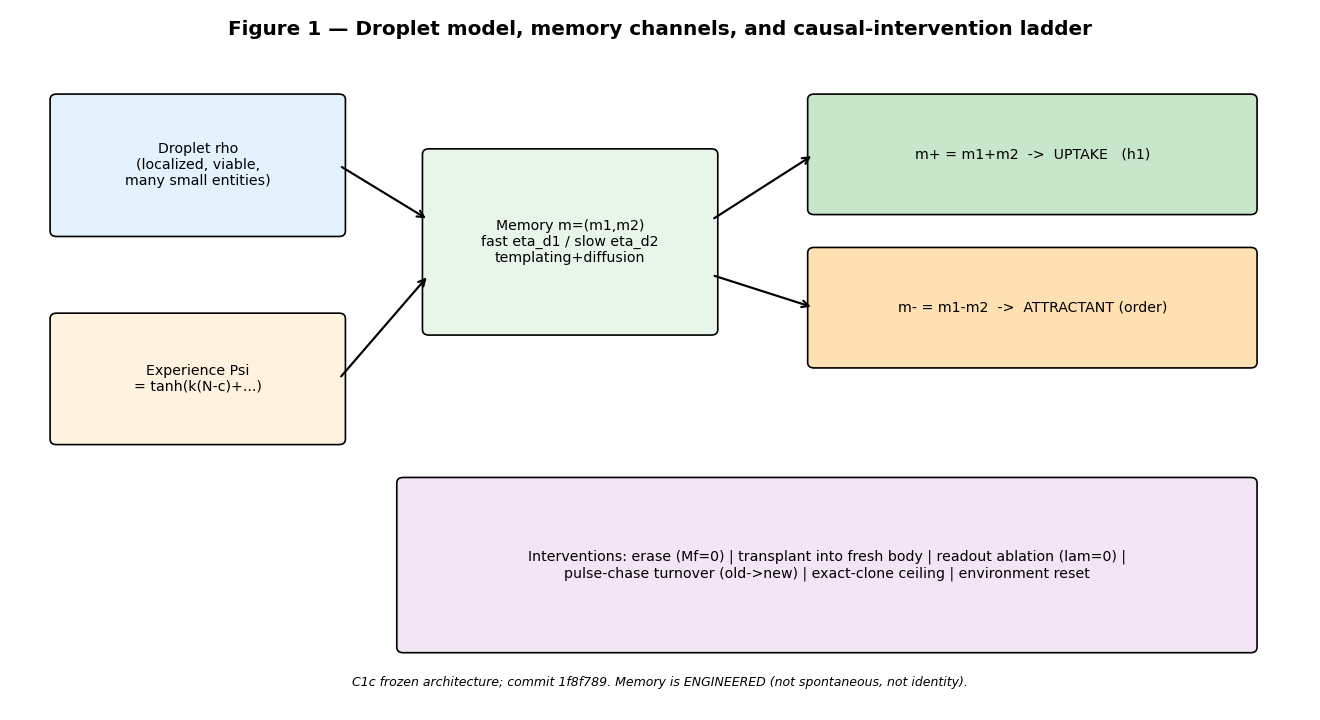
\includegraphics[width=0.86\textwidth]{figs/fig1.png}
\caption{\textbf{Model and causal--intervention ladder (schematic).} Question: what are the write/read pathways and
interventions? Frozen C1c architecture: experience signal $\Psi$ (Eq.~\ref{eq:psi}); two--timescale memory
$m=(m_1,m_2)$ (Eq.~\ref{eq:write}); readouts $m_+\!\to$uptake and $m_-\!\to$attractant
(Eqs.~\ref{eq:readplus}--\ref{eq:readminus}); and the intervention suite (erase, transplant, ablation, pulse--chase,
clone). Schematic; no data. Source: \texttt{docs/paper/fig1\_model\_ladder.png}.}
\label{fig:model}\end{figure}

\begin{figure}[t]\centering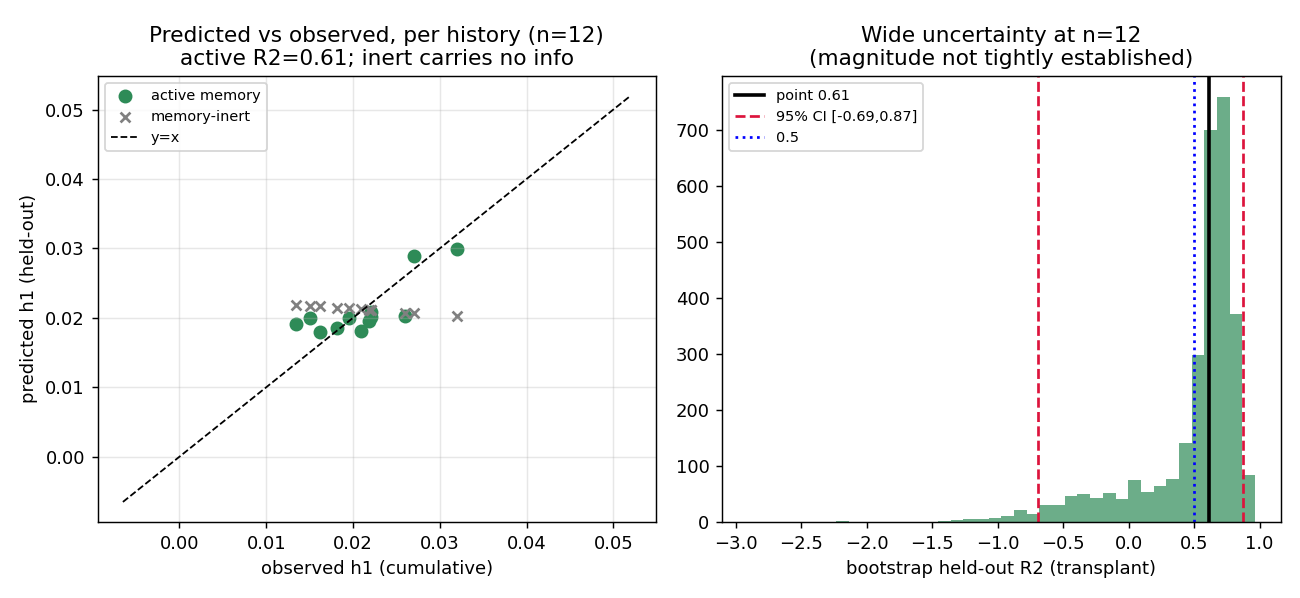
\includegraphics[width=0.55\textwidth]{figs/fig2.png}
\caption{\textbf{$h_1$ causal expression (necessity established; sufficiency magnitude uncertain).} Left: per--history predicted--versus--observed $h_1$ (held--out, $n=12$), for the active memory (green) and the memory--inert control (grey, no information). Right: bootstrap distribution of the transplant $R^2$ (point $0.61$; $95\%$ CI $[-0.69,0.87]$, spanning $0.5$), showing the magnitude is not tightly established at $n=12$. Causal necessity is clean: the inert and erase controls carry no history information (deterministic $R^2=-0.19$). Prospective, grouped leave--history--out; $n_{\text{boot}}=3000$; ridge $\lambda=1$. Data: \texttt{results/wd01\_phasec/phasec\_causal\_*\_raw.pkl}.}
\label{fig:causal}\end{figure}

\begin{figure}[t]\centering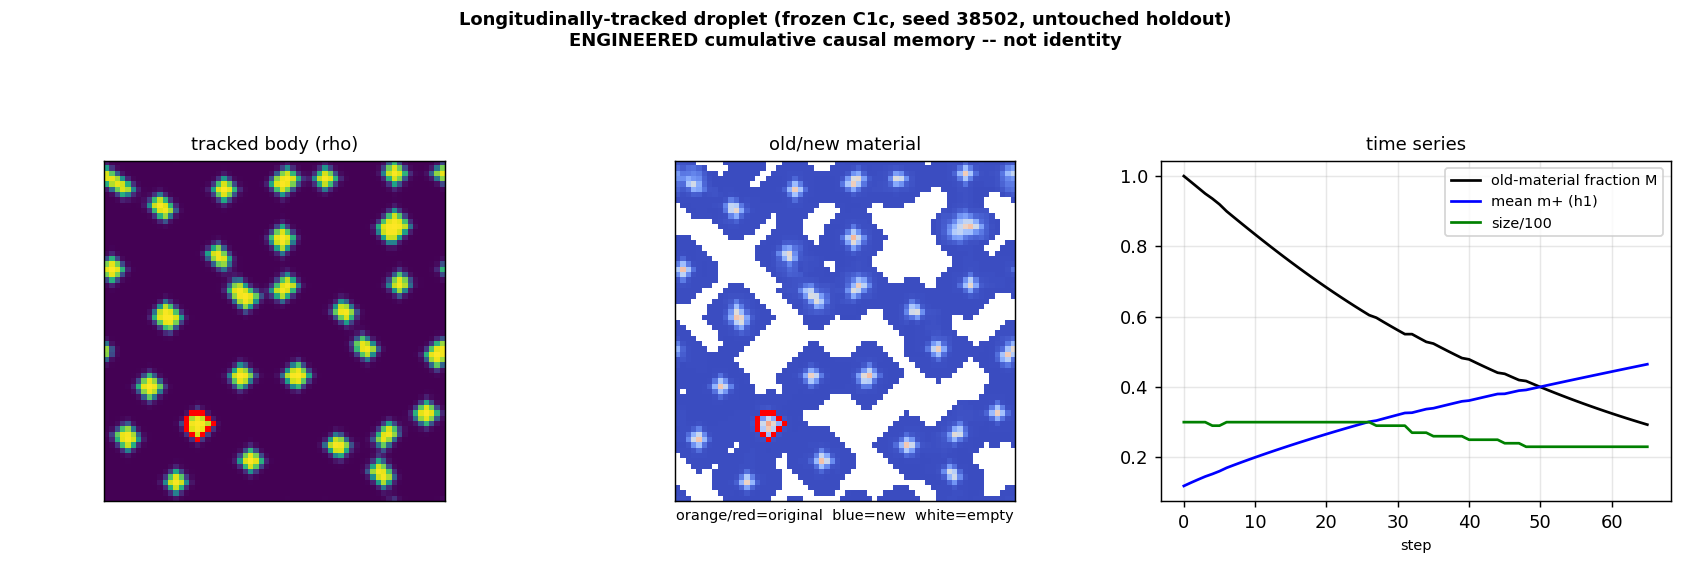
\includegraphics[width=0.95\textwidth]{figs/fig3.png}
\caption{\textbf{Longitudinally--tracked turnover.} Question: does a single tracked droplet retain $h_1$ as its
material is replaced? Protocol: frozen C1c, untouched seed $38502$, longitudinal tracker. The tracked entity (red
contour) is shown on the body panel and, with the \emph{same} contour, on the old/new--material panel
(orange/red $=$ original, blue $=$ new, white $=$ empty); the time series shows old--material fraction $M$
declining, mean $m_+$ ($h_1$) rising, and stable size. Single deterministic trajectory (illustrative);
population certification is Figure~\ref{fig:cert}. Data/script: \texttt{scripts/observe\_droplet.py}.}
\label{fig:track3}\end{figure}

\begin{figure}[t]\centering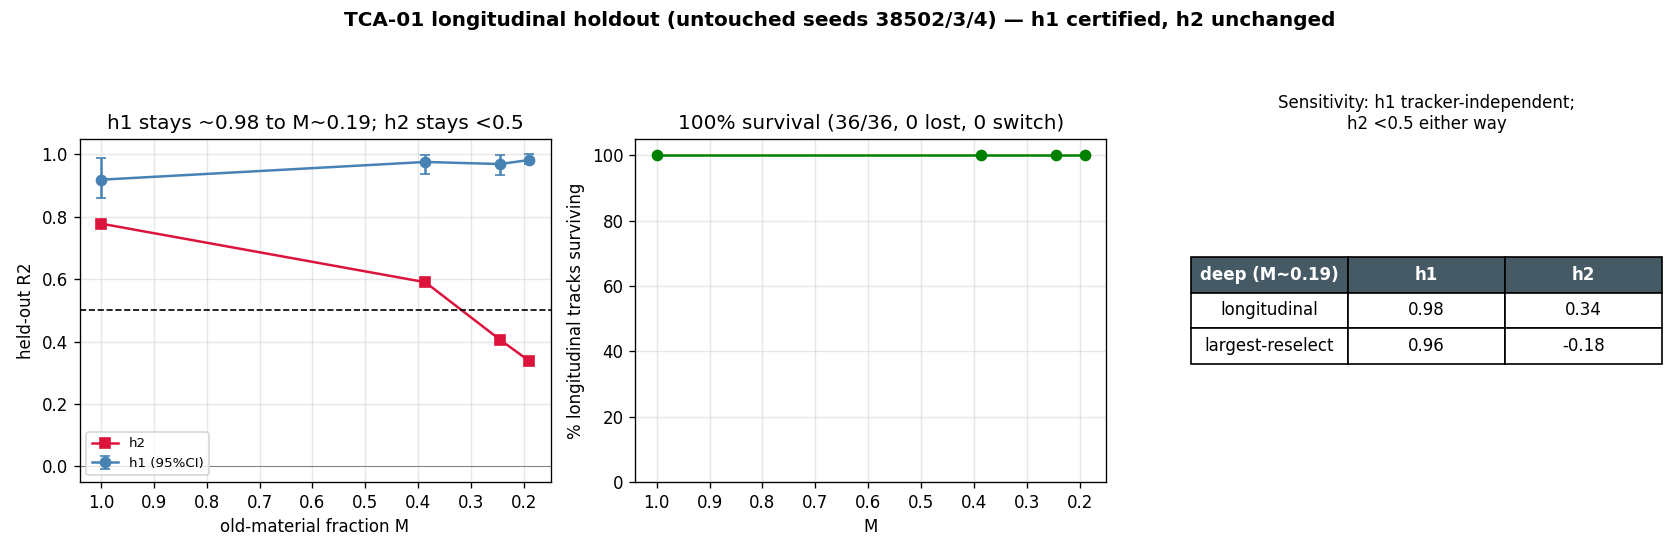
\includegraphics[width=0.95\textwidth]{figs/fig3b.png}
\caption{\textbf{Primary quantitative result: longitudinal hold--out certification.} Untouched sealed seeds $38502$--$38504$, $n=12$ histories
$\times 3$ seeds, executed once. $h_1$ held--out $R^2$ with $95\%$ CI versus $M$ (stays $\approx0.98$ to
$M\approx0.19$); $100\%$ track survival ($36/36$); sensitivity table (largest vs longitudinal). Prospective,
grouped, donor--level bootstrap CIs. Result: $h_1$ certified; $h_2<0.5$. Data: \texttt{results/observer/tca\_holdout\_raw.pkl}.}
\label{fig:cert}\end{figure}

\begin{figure}[t]\centering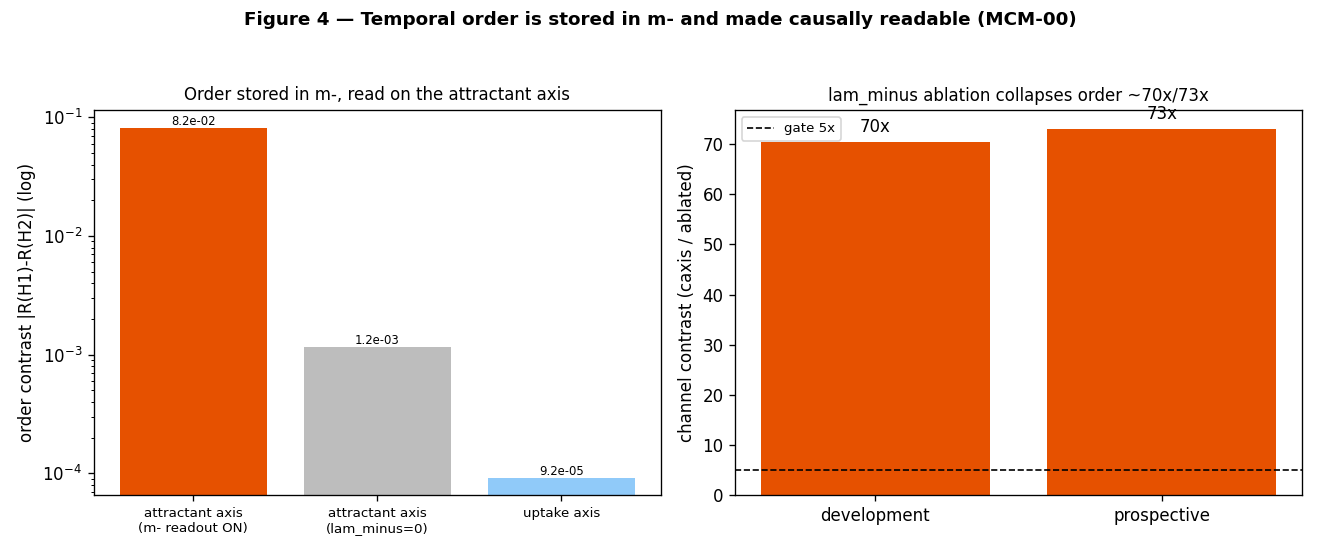
\includegraphics[width=0.95\textwidth]{figs/fig4.png}
\caption{\textbf{Temporal order stored in $m_-$ and made causally readable.} Order contrast on the attractant axis
(readout on) vs $\lambda_-$--ablated vs the uptake axis, and the $\sim$$70$/$73\times$ channel contrast
(development / prospective, $n=16$/$12$). Result: channel--specific order readout; ablation collapses it. Data:
\texttt{results/sc\_mcm/certificate.json}.}
\label{fig:order}\end{figure}

\begin{figure}[t]\centering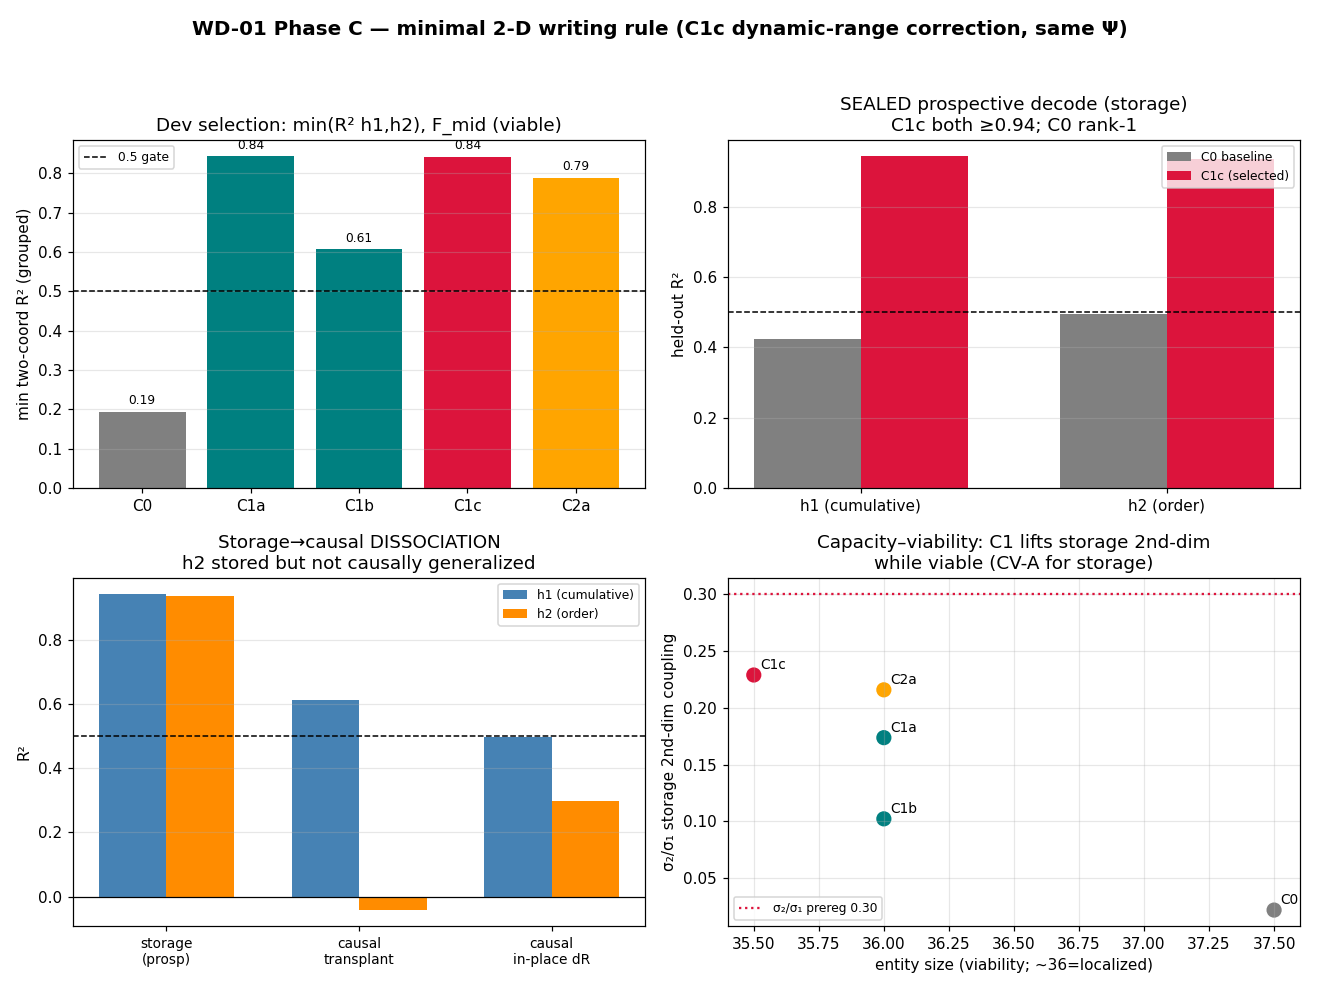
\includegraphics[width=0.95\textwidth]{figs/fig5.png}
\caption{\textbf{Storage versus causal dimensionality.} Two prospectively decodable coordinates at rest with an
$\approx$one--dimensional causal response; the grouped--evaluation correction (row--wise $0.57\to$ grouped $0.19$)
and rank estimators. Prospective, grouped. Data: \texttt{results/wd01\_phasec/*\_raw.pkl}.}
\label{fig:dim}\end{figure}

\begin{figure}[t]\centering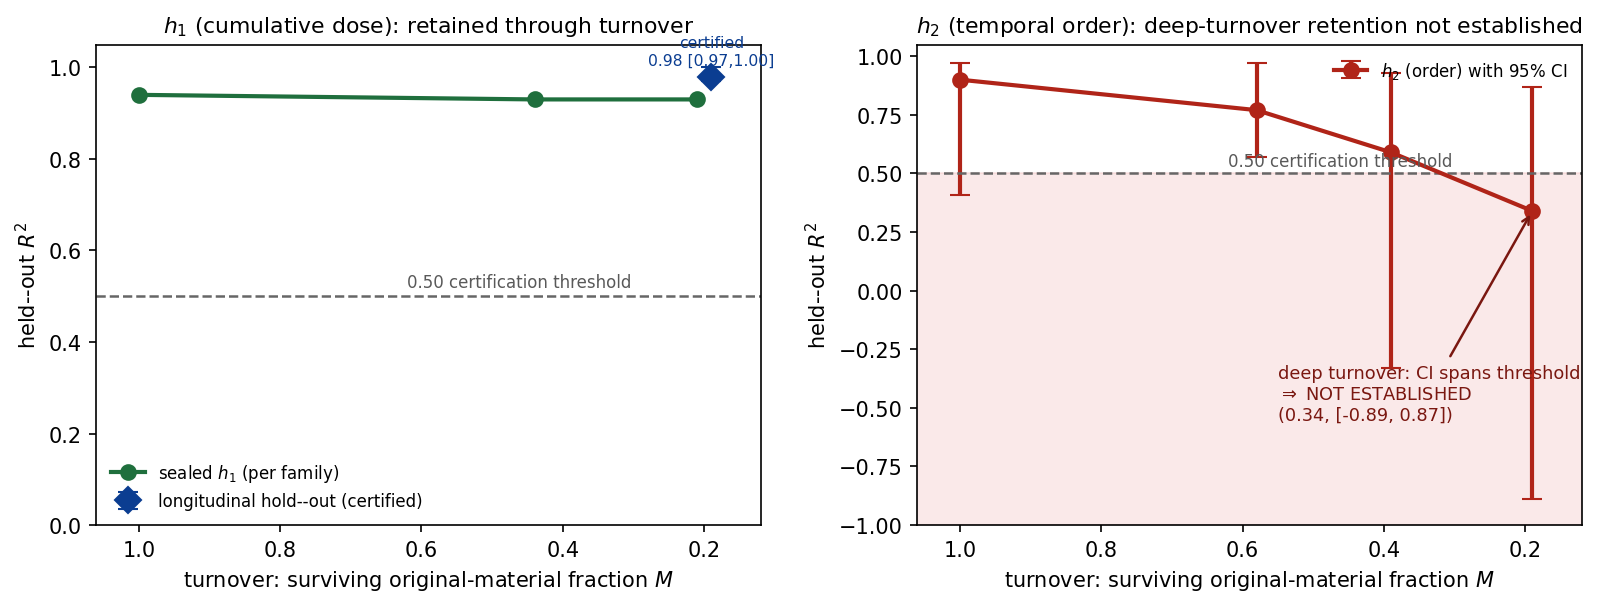
\includegraphics[width=0.98\textwidth]{figs/fig6_killswitch_v3.png}
\caption{\textbf{$h_2$ deep--turnover kill--switch (re--audited).} Held--out decode versus surviving original-material fraction $M$ with $95\%$ bootstrap CIs; dashed line is the $0.50$ certification threshold. \emph{Right:} at deep turnover the corrected longitudinal $h_2=0.34$ has CI $[-0.89,0.87]$ spanning the threshold, so retention is \emph{not established} (a power limit at $n{=}12$, not a demonstrated absence); the original sealed per--frame estimate ($h_2\approx0$) is superseded by the tracker correction (\S\ref{sec:tracker}). \emph{Left:} $h_1$ stays well above threshold across the same turnover and is certified longitudinally. Data: \texttt{results/h2cert/h2cert\_sealed\_raw.pkl}.}
\label{fig:killswitch}\end{figure}

\begin{figure}[t]\centering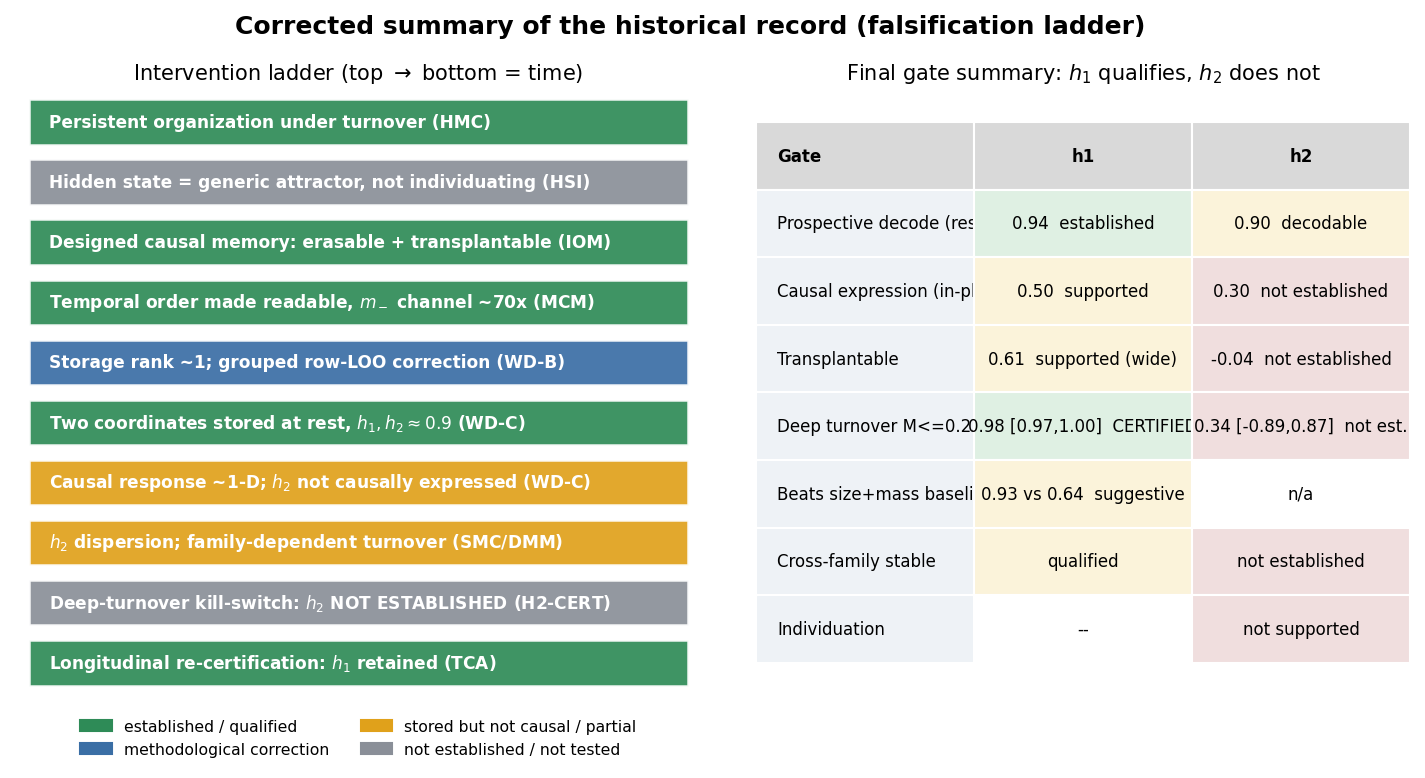
\includegraphics[width=0.95\textwidth]{figs/fig7_claimladder_v3.png}
\caption{\textbf{Corrected summary of the historical record (falsification ladder).} Intervention ladder (qualified / correction /
negative / kill--switch) and the final gate table: $h_1$ qualifies on every gate, $h_2$ does not, individuation
fails. Regenerated with corrected outcomes ($h_2$ deep--turnover shown as \emph{not established}, not failed).}
\label{fig:ladder}\end{figure}


\begin{table}[t]\centering\small
\caption{Development gate outcomes across the ladder (abbreviated).}
\label{tab:gates}
\begin{tabular}{@{}p{3.2cm}p{5.6cm}p{4.6cm}@{}}\toprule gate & criterion & outcome\\\midrule
backward compatibility & $\lambda_-{=}0$ bit--identical to predecessor & pass ($0$ deviation)\\
no tag/tracker leakage & no label in dynamics & pass\\
viability & localized entity through turnover & pass\\
material turnover & passive cohort $M$ decreases & pass\\
storage rank (2nd dim) & $\sigma_2/\sigma_1 \ge 0.30$ (prospective) & marginal fail ($0.283$)\\
$h_1$ deep--turnover (longitudinal) & held--out $R^2\ge0.50$, lower CI${>}0$ & pass ($0.98$, $[0.97,1.00]$)\\
$h_2$ deep--turnover & held--out $R^2\ge0.50$, lower CI${>}0$ & not established ($0.34$, CI $[-0.89,0.87]$)\\
individuation & distinct per--droplet histories decodable & not tested / not supported\\\bottomrule
\end{tabular}
\end{table}
\begin{table}[t]\centering\small
\caption{Post--incident claim corrections (tracker--continuity audit).}
\label{tab:corrections}
\begin{tabular}{@{}ll@{}}\toprule
claim & status after correction\\\midrule
largest--component trajectories as unique continuity & invalidated\\
$h_1$ deep--turnover survival & replaced: longitudinal $0.98$, $[0.97,1.00]$, $36/36$\\
old--material $M$, entity--size time series & replaced by longitudinal\\
``$48/48$ viable'' & qualified: $36/36$ longitudinal survival\\
``a droplet carries memory'' & qualified: a \emph{continuously tracked} droplet\\
tracker--independent decoding & qualified: because $h_1$ is global, not individual\\
transplant / ablation / endpoint causal & unaffected (single--timepoint, common body)\\
$h_2$ turnover failure & unchanged ($0.34<0.50$ longitudinally)\\\bottomrule
\end{tabular}
\end{table}
\begin{table}[t]\centering\small
\caption{Interpretation boundaries: what each result does and does not license.}
\label{tab:boundaries}
\begin{tabular}{@{}p{4.4cm}p{4.4cm}p{4.4cm}@{}}\toprule observation & licenses & does not license\\\midrule
$h_1$ decodable + causal + transplantable & internal causal memory & individual identity\\
$h_1$ survives turnover (longitudinal) & organizational (not material) memory & lineage / heredity\\
$h_1$ global across droplets & memory of shared history & per--droplet private experience\\
$h_2$ decodable at rest & stored variation & causal or persistent memory\\
new material acquires $h_1$ & passive local propagation & active reconstruction\\
kill--switch $h_2$ not established deep ($0.34$, CI spans $0.50$) & a power limit at $n{=}12$ & absence of an order memory\\\bottomrule
\end{tabular}
\end{table}

\section{Discussion}
The ladder is designed to separate concepts that are routinely conflated, and the value of the paper is as much in
the separations as in the final numbers. \emph{Memory versus decodability}: a coordinate that is decodable at rest
($h_2$) need not be a memory in any causal or persistent sense. \emph{Storage versus causal expression}: with the
frozen readouts, two decodable coordinates at rest coexisted with an $\approx$one--dimensional causal response;
storing a number the system cannot act on is not yet functional memory \citep{pearl2009}. \emph{Passive copying
versus reconstruction}: because new material inherits the local intensive memory during growth, propagation of a
coordinate into new material is guaranteed by construction and is \emph{not} evidence of active reconstruction
toward a target. \emph{Material replacement versus organizational inheritance}: $h_1$ information persists in the
internal memory when body size no longer carries it, which is why it exceeds trivial body baselines after turnover.
\emph{Visual/size--reselected continuity versus longitudinal continuity}: a largest--component tracker manufactured
apparent continuity that a longitudinal tracker removes \citep{jaqaman2008,rosenfeld1966}.

What does $h_1$ establish, and what does it not? It establishes that an engineered, bounded internal state can be a
\emph{causal}, \emph{transplantable}, and \emph{turnover--surviving} record of cumulative experience in a persistent
dissipative droplet, certified prospectively on untouched seeds under continuity--safe tracking. It does \emph{not}
establish individual memory. Because the history is imposed globally, $h_1$ is written similarly into every large
droplet, so it is decodable from any of them; its informational content is global even though its storage and causal
expression are local. This is precisely why $h_1$ is robust to the choice of tracker --- and why that robustness
must not be misread as individuation. A genuine individuating memory would require different droplets in one world
to carry \emph{distinct} histories and be distinguishable by them, which our globally driven design does not test
and does not exhibit.

Why did the second dimension fail? $h_2$ is carried by the value--dispersion of the memory, and the maintenance
terms in Eq.~\eqref{eq:write} --- local templating toward a neighbourhood mean and weak diffusion --- are linear
low--pass operators that erode dispersion, while ongoing growth injects fresh, history--independent heterogeneity
that competes with the $h_2$ signal. Molecular memory that survives division uses \emph{bistable}, hysteretic
maintenance \citep{gardner2000,elowitz2000,ferrell2002,ptashne2004}, not linear averaging; our architecture has no
such protection, and a sealed kill--switch (underpowered at $n=12$) did not certify $h_2$ deep--turnover retention: the held--out estimate's $95\%$ confidence interval spans the threshold, so retention is not established rather than confirmed absent. We emphasize that the \emph{mechanism} of $h_2$ non--persistence is not causally identified: disabling the linear smoothing terms individually or together did not change the decode, and the memory dispersion grows rather than shrinks during turnover, which is inconsistent with a simple ``linear averaging erases the code'' account. Growth injecting history--independent dispersion, high between--family variance, and the absence of bistable protection remain \emph{hypotheses}, not established causes.

The methodological contribution generalizes beyond this system. Each rung illustrates a failure mode that recurs in
computational and empirical science: high internal variation mistaken for stored information; row--wise
cross--validation leaking through grouped replicates \citep{kaufman2012}; a single favourable seed family taken as
general; an underpowered estimate at the boundary of a threshold; and a size--based reselection mistaken for
identity tracking. Preregistration, grouped evaluation, sealed hold--outs, kill--switches, and continuity--safe
tracking are the countermeasures, and the paper is in part a worked example of applying them
\citep{nosek2018,popper1959,efron1979}.

Finally, the results speak to the architecture--versus--substrate distinction. We do not claim that the
Particle--Dynamics substrate is incapable of multidimensional organizational memory; we claim that the tested C1c
writing/maintenance/readout architecture did not support a qualified second dimension, and that individuation was
not demonstrated. The substrate--general question remains open, and the failed $h_2$ points to concrete,
non--implemented directions --- active local reconstruction, bistable/epigenetic--like maintenance, or
compartmentalized maintenance --- rather than to a claim of impossibility.

It is worth stating explicitly why the global nature of $h_1$ is not a defect of the experiment but the correct
reading of what was measured. In a world driven by a single global history, the ``memory of experience'' that any
droplet can carry is, at best, a local copy of that shared history; there is no per--droplet private experience to
individuate on. Demonstrating individuation would require a fundamentally different design --- distinct, locally
imposed histories for co--existing droplets in one world, and a decoder that must attribute each droplet's memory to
its own history and not its neighbours'. Our design deliberately does not attempt this, and the tracker--sensitivity
result (identical $h_1$ from different droplets) makes the reason vivid: when the signal is global, following the
``right'' droplet is unnecessary for decoding, which is exactly why it would be necessary --- and currently absent
--- for any individuation claim. The honest conclusion is therefore narrow and, we believe, defensible: an
engineered internal state can be a causal, transplantable, turnover--surviving record of a \emph{shared} history in
a persistent droplet, and this is worth reporting precisely because it stops short of, and clearly delimits, the
stronger claims it is often mistaken for. For the artificial--life programme \citep{bedau2000}, the practical lesson is a checklist for memory claims in simulated organisms: require causal intervention, not decodability; require turnover survival under continuity--safe tracking, not visual persistence; distinguish global from individual information; and preregister a kill--switch so a marginal signal cannot license indefinite mechanism accretion. A qualified second, individuating dimension in this family of models would need three things the present architecture lacks: a second, physically \emph{independent} write signal (so two coordinates are not two filters of one scalar); a \emph{nonlinear, bistable} maintenance rule (so a stored distinction is protected against linear averaging and material renewal) \citep{gardner2000,ferrell2002}; and a design with \emph{distinct per--droplet histories} (so individuation is even testable). None is claimed here. More broadly, we expect the qualitative pattern --- a global, cumulative coordinate surviving turnover while an order/dispersion coordinate does not --- to generalize to related reaction--transport memories with linear maintenance, and we expect the specific corrections (grouped evaluation, continuity--safe tracking, kill--switched escalation) to transfer directly to any simulated--organism study that decodes a history variable from an internal state. What will not transfer without new physics is a positive individuation result: that requires the three missing ingredients above and a design in which co--existing entities carry genuinely distinct histories.

\section{Limitations}
Several limitations bound the interpretation and are stated plainly. First, the memory is \emph{engineered}, not
emergent: we did not show that such a memory arises spontaneously, only that, once present, it is causal and
turnover--surviving. Second, the dynamics are \emph{simulator--specific}; the quantitative thresholds and the
particular maintenance terms are properties of this model, and although the model is in the reaction--diffusion /
active--droplet family \citep{turing1952,zwicker2017}, no claim of quantitative correspondence to a physical protocell
is made. Third, the entities are \emph{small} ($\sim$$30$--$55$ active cells), so per--entity samples are limited and
decoders operate near their statistical floor at deep turnover; the certification survives this, but it is a
constraint. Fourth, the histories are \emph{designed and global}; $h_1$ is consequently low--dimensional and global,
and the design cannot test individuation, which requires distinct per--droplet histories. Fifth, memory is
\emph{explicitly copied} into new material during growth, so ``inheritance'' into new material is by construction,
not reconstruction. Sixth, the causal transplant readout is \emph{mean--field}; a structured transplant that
preserves spatial pattern was not shown to rescue $h_2$, and structured causal expression of a second dimension
remains untested. Seventh, the historical turnover analyses used \emph{largest--component reselection}; we corrected
this and re--certified $h_1$ longitudinally, but the correction narrows the original ``the entity survived'' framing
to ``a continuously tracked droplet retains a global coordinate.'' Eighth, we performed \emph{no reproduction,
budding, or lineage} experiment, and make no heredity or genome claim. Ninth, the second--dimension rank ratio at prospective evaluation ($0.283$) is marginally below the preregistered gate ($0.30$), reported as a strict miss; and the deep--turnover $h_2$ retention is \emph{not established} (its $95\%$ CI spans the $0.50$ threshold at $n=12$), a limitation of statistical power, not a demonstrated absence. The \emph{mechanism} of $h_2$ non--persistence is likewise not causally identified and is left indeterminate. Tenth, the tracker, though frozen and label--free, was developed with knowledge of one incident
trajectory; we mitigated this by certifying on disjoint, untouched seeds, but a fully independent re--seal would
further strengthen the claim.

\section{Conclusion}
Under a globally imposed history, many persistent simulated droplets locally encode a similar engineered
one--dimensional cumulative causal memory; a continuously tracked droplet retains this internal causal state through
substantial constituent turnover ($h_1$ held--out $R^2=0.98$, $[0.97,1.00]$, at $M\approx0.19$, $36/36$ survival),
; its causal expression is established in necessity (inert/erase controls carry no information) with an uncertain sufficiency magnitude. This memory does not individuate droplets: its informational content
is global even though storage and causal expression are local. A second, initially decodable coordinate was \emph{not established} as an independent, causal, turnover--surviving dimension: its deep--turnover held--out estimate carries a confidence interval spanning the certification threshold, so it is neither confirmed nor refuted at the sample size we ran.
We report these boundaries --- and the corrections required to reach them --- as the result. Individuation,
reproduction, and a genome are not warranted by the present evidence.

\section*{Author contributions}
[AUTHOR NAME REQUIRED] designed and performed the simulations and analyses and wrote the manuscript. Author
identity, affiliation, and ORCID are placeholders pending the corresponding author's confirmation.

\section*{Competing interests}
The author declares no competing financial or non--financial interests.

\section*{Funding}
[FUNDING STATEMENT REQUIRED --- no external funding is asserted.]

\section*{AI-assistance disclosure (draft)}
An AI system (an autonomous coding/analysis agent) assisted with implementation, statistical analysis, figure
generation, the tracker--continuity audit, and drafting under human direction. All scientific claims trace to
committed code and data; the human author is responsible for the content. This disclosure is a draft for adaptation
to the target venue's policy.

\section*{Data and code availability}
All code, frozen configurations, sealed prospective manifests (SHA--256), raw data, analysis scripts, and figure
generators are retained under isolated version--control branches (Supplement). Negative results and corrections are
preserved. All code, configurations, manifests, and raw data are committed in the project repository at the exact commit hashes listed in the Supplement; no public archive has yet been released (a release checklist is provided), and access should be requested from the authors until a public deposit is made. No data relevant to the reported analyses were excluded.

\section*{Threats to validity and robustness}
We enumerate the residual threats and how each is addressed. \emph{Selection on the prospective family}: sealed
families are hashed before selection and executed once; the deep--turnover certification uses seeds never inspected
during tracker development. \emph{Multiple comparisons}: the ladder is a fixed sequence of preregistered gates, not
a search over many decoders; the single primary metric at each rung is declared in advance. \emph{Decoder
flexibility}: the primary decoder is a transparent regularized linear model, and nonlinear decoders are used only as
secondary diagnostics, because a sufficiently flexible decoder can recover a target from nuisance structure and
thereby manufacture a false positive. \emph{Grouping}: all replicate rows sharing a history, a donor, a clone, or a
trajectory prefix are held out together. \emph{Tracker post--selection}: the longitudinal tracker uses only
geometric overlap and is certified on disjoint untouched seeds. \emph{Small samples}: the deep--turnover estimates
are the weakest link, and we report their wide confidence intervals honestly rather than a point estimate; the
$h_1$ certification survives this scrutiny because its lower bound is far from the threshold, whereas the $h_2$ result is inconclusive at this sample size: its interval spans the threshold, so deep--turnover retention is not established rather than shown absent.

\section*{Reproducibility statement}
Physics is frozen (Table~\ref{tab:params}); sealed families were hashed before selection and executed once
(Table~\ref{tab:families}); decoding uses grouped leave--history--out cross--validation to avoid replicate leakage;
the longitudinal tracker is frozen and label--free. Per--experiment run commands and hashes are in the Supplement.

\bibliographystyle{unsrtnat}
\bibliography{references}
\end{document}
